
\chapter{用有限信息进行三维形状识别的深度时空网络}

在过去几年的相关工作创造性地提出了一些基于深度学习的三维形状描述符,它们具有很强的学习高层次特征的能力,但其中大部分只是使用深度学习方法来提取高层特征,而忽略获取信息的时空关系。以至于捕获的视图分别被训练和使用。为了使三维形状识别与检索系统适用于移动机器人与环境的自主交互,需要使用模仿人的空间相关图像来实现高精度的物体识别。在本文中,我们提出了一种新的三维形状识别和检索框架,它通过记忆机制同时学习高级特征和对时空信息进行建模。本文提出了一种新颖的三维形状识别与检索框架,结合卷积神经网络(CNNs)和长短期记忆(LSTM),学习了三维物体视觉信息的时空序列关系。具体而言, CNNs是“视觉系统”,因为它具有强大的提取有效视觉特征的能力,而LSTM是“记忆系统”,因为该模型可以学习不同视觉特征的时空顺序关系。大量的实验表明,所提出的框架对使用有限的序列信息能够获得较好的性能。

虽然前面提到的几何,视觉和深度学习三种方法在计算机图形学界已经做出了很大的贡献,但是对于在真实环境中识别三维物体的移动机器人来说,还远远不能令人满意。 首先,移动机器人应该以较少的视角做出快速准确的判断,这就要求视角特征的高质量。其次,大多数现有的形状描述符忽略了连续帧探测的信息。 这两个问题限制了机器人在真实复杂的世界中实现自由操作。 综合考虑,本文提出了一个新的框架,它包含两个过程,即基于视图的描述符生成和基于记忆的时空信息建模。

\begin{figure*}[tbh]
\begin{center}
 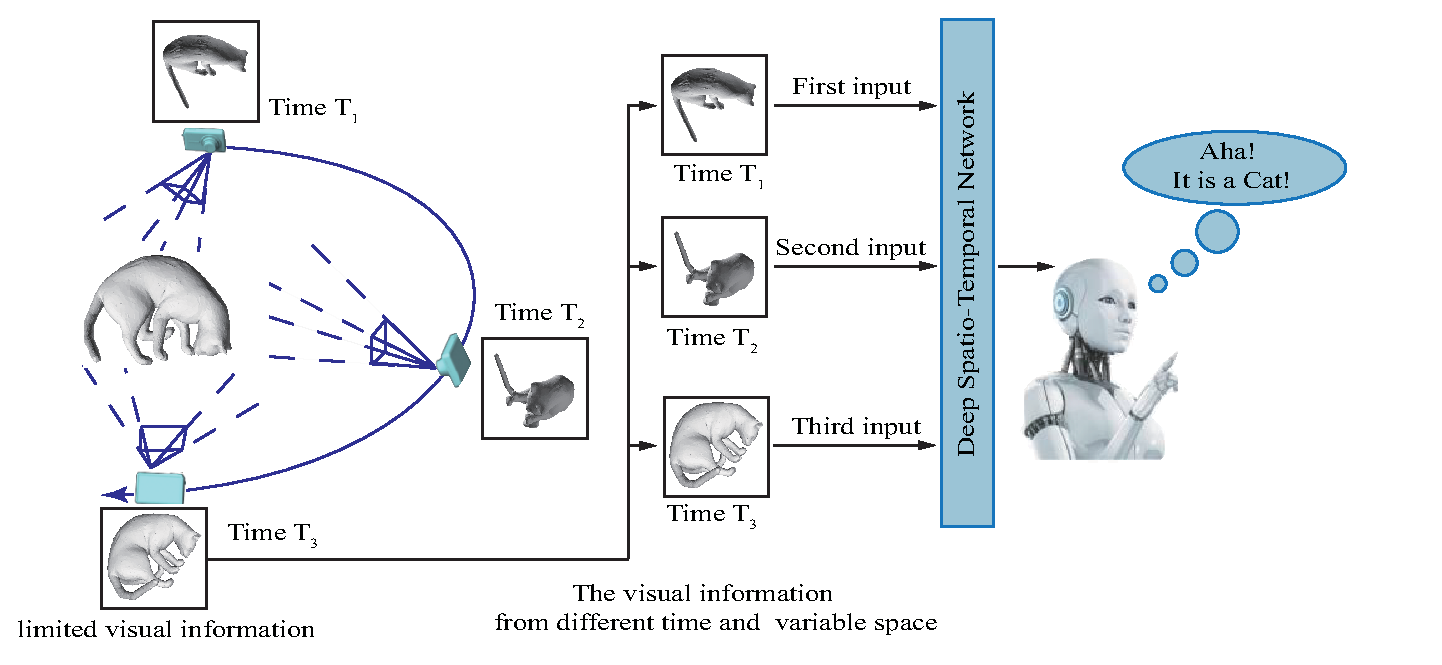
\includegraphics[width=0.98\linewidth]{figures/flowchart.eps}
 \end{center} \vspace{-4mm}
\caption{三维形状的深度时空网络} 
\label{flowchart4}
\end{figure*}

本节提出的方法流程图如图\ref{flowchart4}所示,展示了CNN和LSTM生成的深层时空特征的框架。 在生成二维投影的过程中,由于深度相机以一定的顺序拍照,投影包含一定的时空序列关系。在视觉特征提取中,我们以深度图像为输入,不需要下采样。为了探索二维图像的时空顺序关系,我们的方法是利用LSTM模型的顺序数据学习能力。我们引导LSTM具有监督学习结构,学习的三维形状表示。每一步的细节如下。

\section{所涉及的深度学习方法介绍}
\textbf{长短期记忆网络(LSTM)}
中文分词、词性标注、命名实体识别、机器翻译、语音识别都属于序列挖掘的范畴。序列挖掘的特点就是某一步的输出不仅依赖于这一步的输入,还依赖于其他步的输入或输出。在序列挖掘领域传统的机器学习方法有HMM(Hidden Markov Model,隐马尔可夫模型)和CRF(Conditional Random Field,条件随机场),近年来又开始流行深度学习算法RNN(Recurrent Neural Networks,循环神经网络)。

\textbf{循环神经网络 (RNN)}

CNN等传统神经网络的局限在于:将固定大小的向量作为输入(比如一张图片),然后输出一个固定大小的向量(比如不同分类的概率)。不仅如此,CNN还按照固定的计算步骤(比如模型中层的数量)来实现这样的输入输出。这样的神经网络没有持久性:假设你希望对电影中每一帧的事件类型进行分类,传统的神经网络就没有办法使用电影中先前的事件推断后续的事件。
RNN 是包含循环的网络,可以把信息从上一步传递到下一步。

RNN的循环展开之后其实就是同一个网络复制多份,次序连接进行信息传递。RNN允许信息的持久化,对当前的状态保留记忆(以隐变量的方式存在,也就是图中计算$h_{t}$需要用到$h_{t-1}$的信息)。对于同一个RNN来说,其“A结构”(绿色部分)是固定的(共享一套参数,毕竟是从循环展开来的啊肯定是一样的)。

\textbf{RNN弊端和LSTM}
RNN 是在有顺序的数据上进行学习的. 为了记住这些数据, RNN 会像人一样产生对先前发生事件的记忆。 在反向传递得到的误差的时候, 他在每一步都会 乘以一个自己的参数 W。如果这个 W 是一个小于1 的数, 比如0.9. 这个0.9 不断乘以误差, 误差传到初始时间点也会是一个接近于零的数, 所以对于初始时刻, 误差相当于就消失了。 我们把这个问题叫做梯度消失或者梯度弥散 Gradient vanishing. 反之如果 W 是一个大于1 的数, 比如1.1 不断累乘, 则到最后变成了无穷大的数, RNN被这无穷大的数撑死了, 这种情况我们叫做剃度爆炸, Gradient exploding. 这就是普通 RNN 没有办法回忆起久远记忆的原因.

因为RNN的信息只能传递给相邻的后继者(从循环展开之后的表示来看),因此当输出与其相关的输入信息相隔较近的时候,普通的RNN是可以胜任的。而当这个间隔很长的时候,虽然理论上RNN是可以处理这种长期依赖 (Long Dependencies) 的问题,但是实践中并没有成功。Bengio, et al. (1994)等人对该问题进行了深入的研究,他们发现了使训练 RNN 变得非常困难的根本原因(梯度消失/梯度爆炸)。相关信息输入与需要该信息的输出之间间隔很长。因此,Hochreiter和Schmidhuber (1997)提出了Long Short Term Memory 网络 (LSTM),并在近期被Alex Graves进行了改良和推广。



\section{CNN提取视觉描述符}

从视角来分析3D形状的流行方式是将3D模型从各个角度转换成2D图像。 理论上,这些二维图像应尽可能包含来自三维模型的信息。 在我们的视觉描述符生成过程中,我们首先将三维形状投影到二维图像中,并采用CNN进一步提取视觉特征。 我们的算法的细节总结如下。

\textbf {3D模型预处理。} 在这部分中,我们将原点设置在三维模型质心的中心,然后测量点的最大极距到其表面上的一个点。 虽然没有旋转归一化,但是这将在后面一定程度上被补偿。

\textbf{深度图像的采集。} 深度图像,一种二维图像,来自于从质心居中的正十二面体的20个顶点的虚拟相机的拍摄。在所提出的方法中,我们旋转正十二面体10次以使该特征对旋转具有鲁棒性。应该仔细设置旋转角度,以确保所有相机均匀分布,并能够覆盖3D模型的不同视角。 我们认为十二面体有20个顶点可以产生中等数据量,从而保证高计算性能和重要的信息。 该策略与LFD在视图提取方面类似,但略有不同,我们丢弃二值图像,只使用二维深度图像。 最后一个3D模型由200个图像表示,每个图像的大小为256×256。
\begin{figure*}[tbhp]
\begin{center}
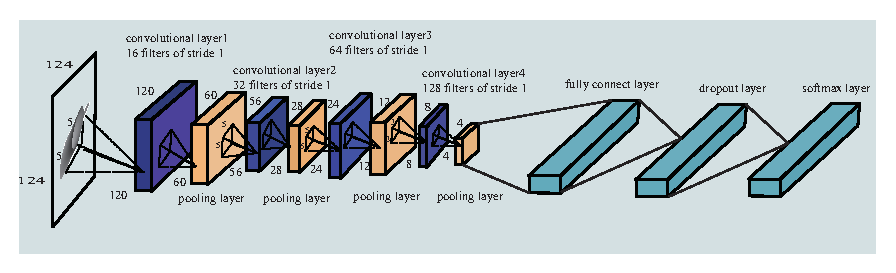
\includegraphics[width=0.9\linewidth]{figures/CNN_LSTM_view.eps}
\end{center} 
\vspace{-4mm}
\caption{我们的3D形状CNN模型的结构。为了说明的目的,我们只为每个卷积层绘制一个滤波器。 从单个视图中提取视觉特征,CNN有着完美的表现。} \label{fig_CNN_view}
\end{figure*}
在深度图像渲染中,有效信息集中在图像的中心。 因此,我们移除深度图像的边界,并将图像从256×256裁剪成124×124的大小,以滤除干扰和冗余信息,从而使数据紧凑。 另外,由于图像尺寸小于原始深度图像,该处理可以促进之后的CNN特征学习。 因为CNN模型的有效输入范围是从0到1,所以深度图不适合作为CNN模型的输入。 因此,我们将每个维度的范围标准化为[0,1]。



\textbf {视觉描述符。} CNN是一种功能强大的深度学习技术,在计算机视觉领域取得了很好的图像特征提取。从上面的程序中,我们获得包含丰富的关于3D模型的视觉信息的2D图像。因此,CNN被用来提取3D形状的每个图像的视觉特征。如图\ref{fig_CNN_view}所示,CNN由4个卷积层组成,其后是一个完全连接层,一个dropout层和一个softmax分类层用于提取二维图像的特征。对于每个卷积层$ l $,我们有:
%
\begin{equation}
	\mathbf{F}_l = pool(ReLU(\mathbf{W}_l * \mathbf{F}_{l-1} + \mathbf{b}_l)),
\label{cal_CNN}
\end{equation}
%
其中$ l\in \{1,...,4 \} $,$ \mathbf {b} _l$是$ l $ -th层的偏置参数,$ \mathbf {W} _l $是卷积核。初始特征图是2D图像$ \mathbf {F}_0 $。整流线性单位(ReLU)激活函数是阈值函数,当变量小于0时为零,然后当变量大于0时与斜率1呈线性关系。池操作是考虑激活的邻域并在每个激活中产生激活函数。 Max-pooling算子是该作品池函数,它在邻域内得到最大的数值被激活,并给平移带来内置的不变性。CNN网络由四个卷积层组成。滤波器的数目从1 $ st $到最后一个卷积层设置为16,32,64,128,所有图层的滤波器大小分别设置为5,5,5,3。所有pooling层大小设置为2.在网络末端增加了dropout层,以避免过度拟合。在这个框架下,我们使用反向传播方法,输入为3D形状的深度图像和相应的标签。在完成CNN模型训练之后,对于每个输入深度图像,使用CNN的正向公式生成相应的视觉描述符$o(\mathbf{X}_{2D})$。

一般来说,视觉描述符对于三维形状识别任务是不够的,因为三维形状只从一个角度不能完全表示三维形状。 作者发下视觉描述符的时空顺序关系被忽略。 因此,作者探索不同视点的时空序列关系,进一步挖掘三维模型的内在特征。

\section{LSTM提取深度时空特征}

传统的神经网络很少学习序列信息,这似乎是一个主要的缺陷。递归神经网络解决了这个问题,即网络中存在循环,并允许信息持续存在。 传统的递归神经网络通过将输入序列映射到隐藏状态以及隐藏状态通过以下等式来输出时间动态模型:
%
\begin{equation}
 h_{t} = g(W_{xh}*x_{t} + W_{hh}*h_{t-1} + b_{h}),
\end{equation}
%
\begin{equation}
 z_{t} = g(W_{hz}*h_{t} + b_{z}) .
\end{equation}
%
其中g是元素非线性,$h_t \in R^N$是包含$N$个隐藏单位的隐藏层,$ z_t $是时间$ t $的输出。 对于长度为$ T $的输入序列$ <x_1,x_2,...,x_T> $,上面的更新按$h_1$ ($h_0 = 0$),$z_1, h_2, z_2, ..., h_T, z_T$的顺序计算。 尽管RNN在语音识别和文本生成等任务中已经证明是成功的,但是要培养他们学习长期动态性还是很困难的。 LSTM提供了一个解决方案,通过结合记忆单元,明确允许网络学习何时“忘记”以前的隐藏单元,何时更新隐藏状态,给出新的信息。过程的细节如下。

\textbf {输入预处理}。 在LSTM体系结构中,序列长度根据输入数据的序列大小而变化。 在我们的框架中,我们对LSTM体系结构采用不同的序列长度来学习3D形状的多视图特征。

\begin{figure*} [htbp]
\begin{center}
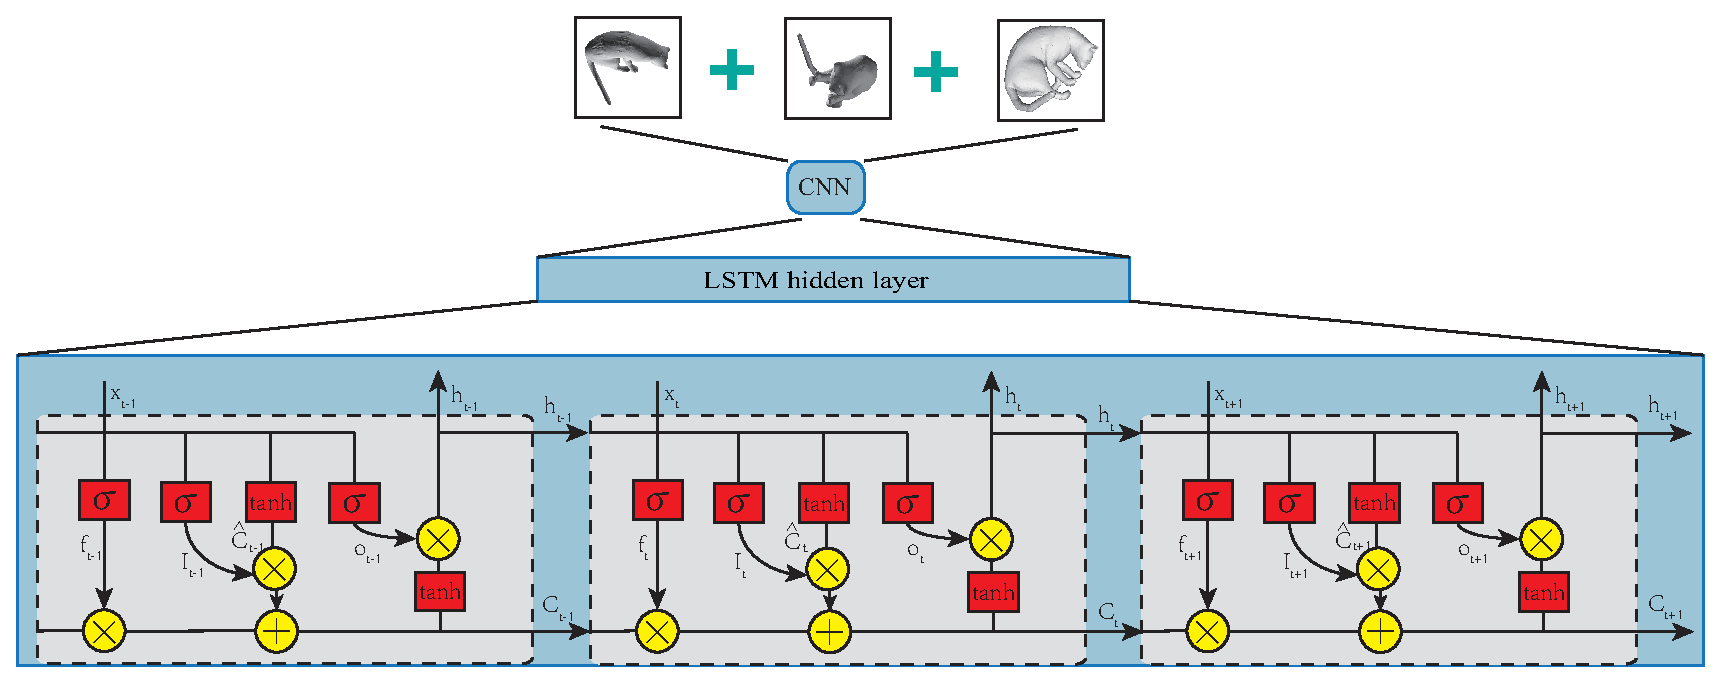
\includegraphics[width=0.98\linewidth]{figures/CNN_LSTM_lstm.eps}
\end{center} 
\vspace{-4mm}
\caption{我们的LSTM模型的体系结构。 为了说明的目的,我们只用三个多视图的三个步骤。 LSTM模型具有很强的学习三维形状学习不同视角的隐藏时空序列信息的能力。 }
\label{fig_lstm}
\end{figure*}

\textbf {时空描述符}。 随着对LSTM的研究的深入,已经提出了在记忆单元内多个不同连接的隐藏单元。 我们使用LSTM单元如下。 如图\ref{fig_lstm}所示,LSTM的存储单元包含四个主要部分,包括输入门,自回归神经元,忘记门和输出门,这些被用来提取时空的顺序关系。 当我们提供多视图特征$ x_t $作为LSTM的输入时,在输入门激活时,候选值$ \hat {C}_t $和记忆单元处的激活部分可以被计算为:
\begin{eqnarray}
 I_t =  \sigma \left( W_Ix_t + H_Ih_{t-1} + b_I\right), \\
 \hat{C}_t =  tanh(W_cx_t + H_ch_{t-1} + b_c), \\
 f_t = \sigma(W_fx_t + H_fh_{t-1} + b_f).
\end{eqnarray}
%
其中$ \sigma(x)$是一个sigmoid层,它决定有多少信息通过这个层并输出$ O_\sigma \in(0,1] $,同时$ \sigma(x) = (1 + e^{-x})^{-1}$ 是非线性的S函数。令$ tanh(x)= \frac {e ^ x-e ^ { - x}} {e ^ x + e ^ { - x}} = 2 \sigma(2x)-1 $是双曲正切非线性, 其输入到[-1,1]范围内。遗忘门通过决定应该忘记多少信息来确定新的单元状态$ C_t $。给出输入门激活$ I_t $的值,忘记门激活$ f_t $和候选值$ \hat {C} _t $,新的单元格状态$ C_t $可以使用下面的方法获得:
%
\begin{equation}
  C_t = f_t * C_{t-1} + I_t * \hat{C}_t.
\end{equation}
%
然后可以基于输入$ x_t $获得输出门控值$ o_t $,该输入$ x_t $是前一时间步骤$ h_ {t-1} $的隐藏层值,并且更新后的单元状态值$ C_t $ 通过:
%
\begin{equation}
  o_t = \sigma(W_ox_t + H_oh_{t-1} + b_o).
\end{equation}
%
新的隐藏层的值$ h_t $可以使用下面的公式计算:
\begin{equation}
  h_t = o_t*tanh(C_t).
\end{equation}
在上述公式中,$ W_I,W_c,W_f,W_o,H_I,H_c,H_f,H_o $是模型的权重参数,$ b_I,b_f,b_c,b_o $是偏差向量。

LSTM用于学习具有不同视觉描述符$o(\mathbf{X}_{2D})$的三维时空特征$h(\mathbf{X}_{3D})$。时间步长根据时空序列的大小设置。交叉熵被定义为损失函数。 优化函数是学习率为0.001的梯度下降算法。对于识别任务,在学习的3D特征上使用softmax回归来执行“一对多”分类。 对于检索任务,利用3D特征的$ L_2 $距离来测量两个形状$ \mathbf {X} $和$ \mathbf {Y} $的相似度
\begin{equation}
 d_s(\mathbf{X}, \mathbf{Y}) = || h(\mathbf{X}_{3D}) - h(\mathbf{Y}_{3D}) ||_2 
 \label{cal_cal_distance}.
\end{equation}


\section{实验}
我们使用了包括SHREC-2015基准\cite {Lian2015SHREC},SHREC 2011非刚性3D水密数据集\cite {Lian2011SHREC},SHREC 2007水密模型\cite {giorgi2007watertight},McGill shape benchmark \cite {zhang2005retrieving} 评估所提出的方法在分类和检索任务中的性能。

SHREC-2015基准是一个三维形状的数据集,由来自50个类的1200个网格模型组成,每个类包含24个具有不同姿势的模型。 SHREC2011非刚性数据集由从30个原始模型转换而来的600个三角形网格组成。 SHREC2007防水数据集由400个网格模型组成,分为20个类别,每个类别包含20个具有不同几何变化的形状,也包含关节变形。数据集不仅包含自然物体,还包含人造物体。 McGill形状基准包含457个模型,包括具有铰接部件和无铰接的形状。 这组关节形状由10个类别中的255个模型组成,每个类别有20个$ sim $ 30个模型。

代码的主要部分是用Python编写的,代码的一部分是用C ++编写的,我们用TensorFlow来构造CNN和LSTM这样的深度学习模型。TensorFlow是一个开源的软件库,用数值流图 研究人员很容易进行机器学习和深度神经网络研究。

\begin{table}[tbhp]
\caption{平均分类结果(\%)}\label{table_classification_results}
\begin{center}
\begin{tabular}{lcccc}  % {lccc} c
\hline \hline	
Method      &SHREC 		&SHREC		&SHREC          & McGill \\ 
            & 2015		& 2011			& 2007		& \\
\hline					
Only CNN feature		&88.90	    	&89.20  			&92.58				  &92.62 \\
\hline
DSTF with 3 views  							&96.61 			&95.98				&97.00          	  &97.80  \\
\hline 
DSTF with 200 views 							&99.00			&97.66				&98.75				  &99.56  \\
\hline  \hline   
\end{tabular}
\end{center} 
\end{table}


\subsection{网络设计}
回顾整个框架,网络架构对于取得好的表现是非常重要的。首先,在学习CNN描述符的步骤中,CNN中的卷积层数会影响识别精度和计算速度。层数越多,分类精度越高,但速度慢,同时层数少,速度越快,但精度低。在我们的工作中,随着层数的增加,计算速度将大大下降,导致计算性能低下,分类的准确性不再明显提高。为了在计算速度和分类精度上取得良好的性能,我们选择4层作为CNN的适当层数。而且,层数与数据集的规模有关。小数据集不能完全训练有很多层的模型。因为数据集的规模不是很大,不适合很深的层次。为了避免整个CNN模型过拟合,我们在模型的末尾添加了dropout层。在初始化CNN模型的权重和偏差的过程中,应该添加一些噪声来打破对称性,避免零梯度。此外,由于CNN模型采用整流线性单位激活函数ReLU,因此最好使用较小的正数初始化偏置项。其次,在LSTM模型中,隐藏节点数对性能也是至关重要的。 一般情况下,如果设置较大的隐藏节点数量来获取丰富的时序信息,分类精度较高; 但计算效率较低。 为了达到平衡性能,我们选择256个隐藏节点作为中等大小。

\subsection{分类实验}
测试形状分类实验以评估特征是否有资格正确分类形状集合。将平均分类准确度作为以下实验的评估度量。对于三个形状基准的每个数据集,我们随机选择每个类别的50%模型作为训练样本,其余模型作为测试数据。

我们在SHREC2015,SHREC2011,SHREC2007和McGill数据集上进行分类实验。 实验的平均分类准确性在表\ref {table_classification_results}中被观察到。 从表\ref{table_classification_results}中,我们可以清楚地得出结论,SPF比只有CNN功能要好。 而且,使用的视图越多,获得的性能越好。 此外,由于分类精度高,所提出的方法具有很强的呈现三维形状的能力。 这可以用以下两个事实来解释:来自三维形状的CNN描述符具有很强的区分两个模型之间差异的能力,并且LSTM模型利用这些CNN描述符挖掘时空顺序关系。

\begin{figure*}[tbhp]
\begin{center}
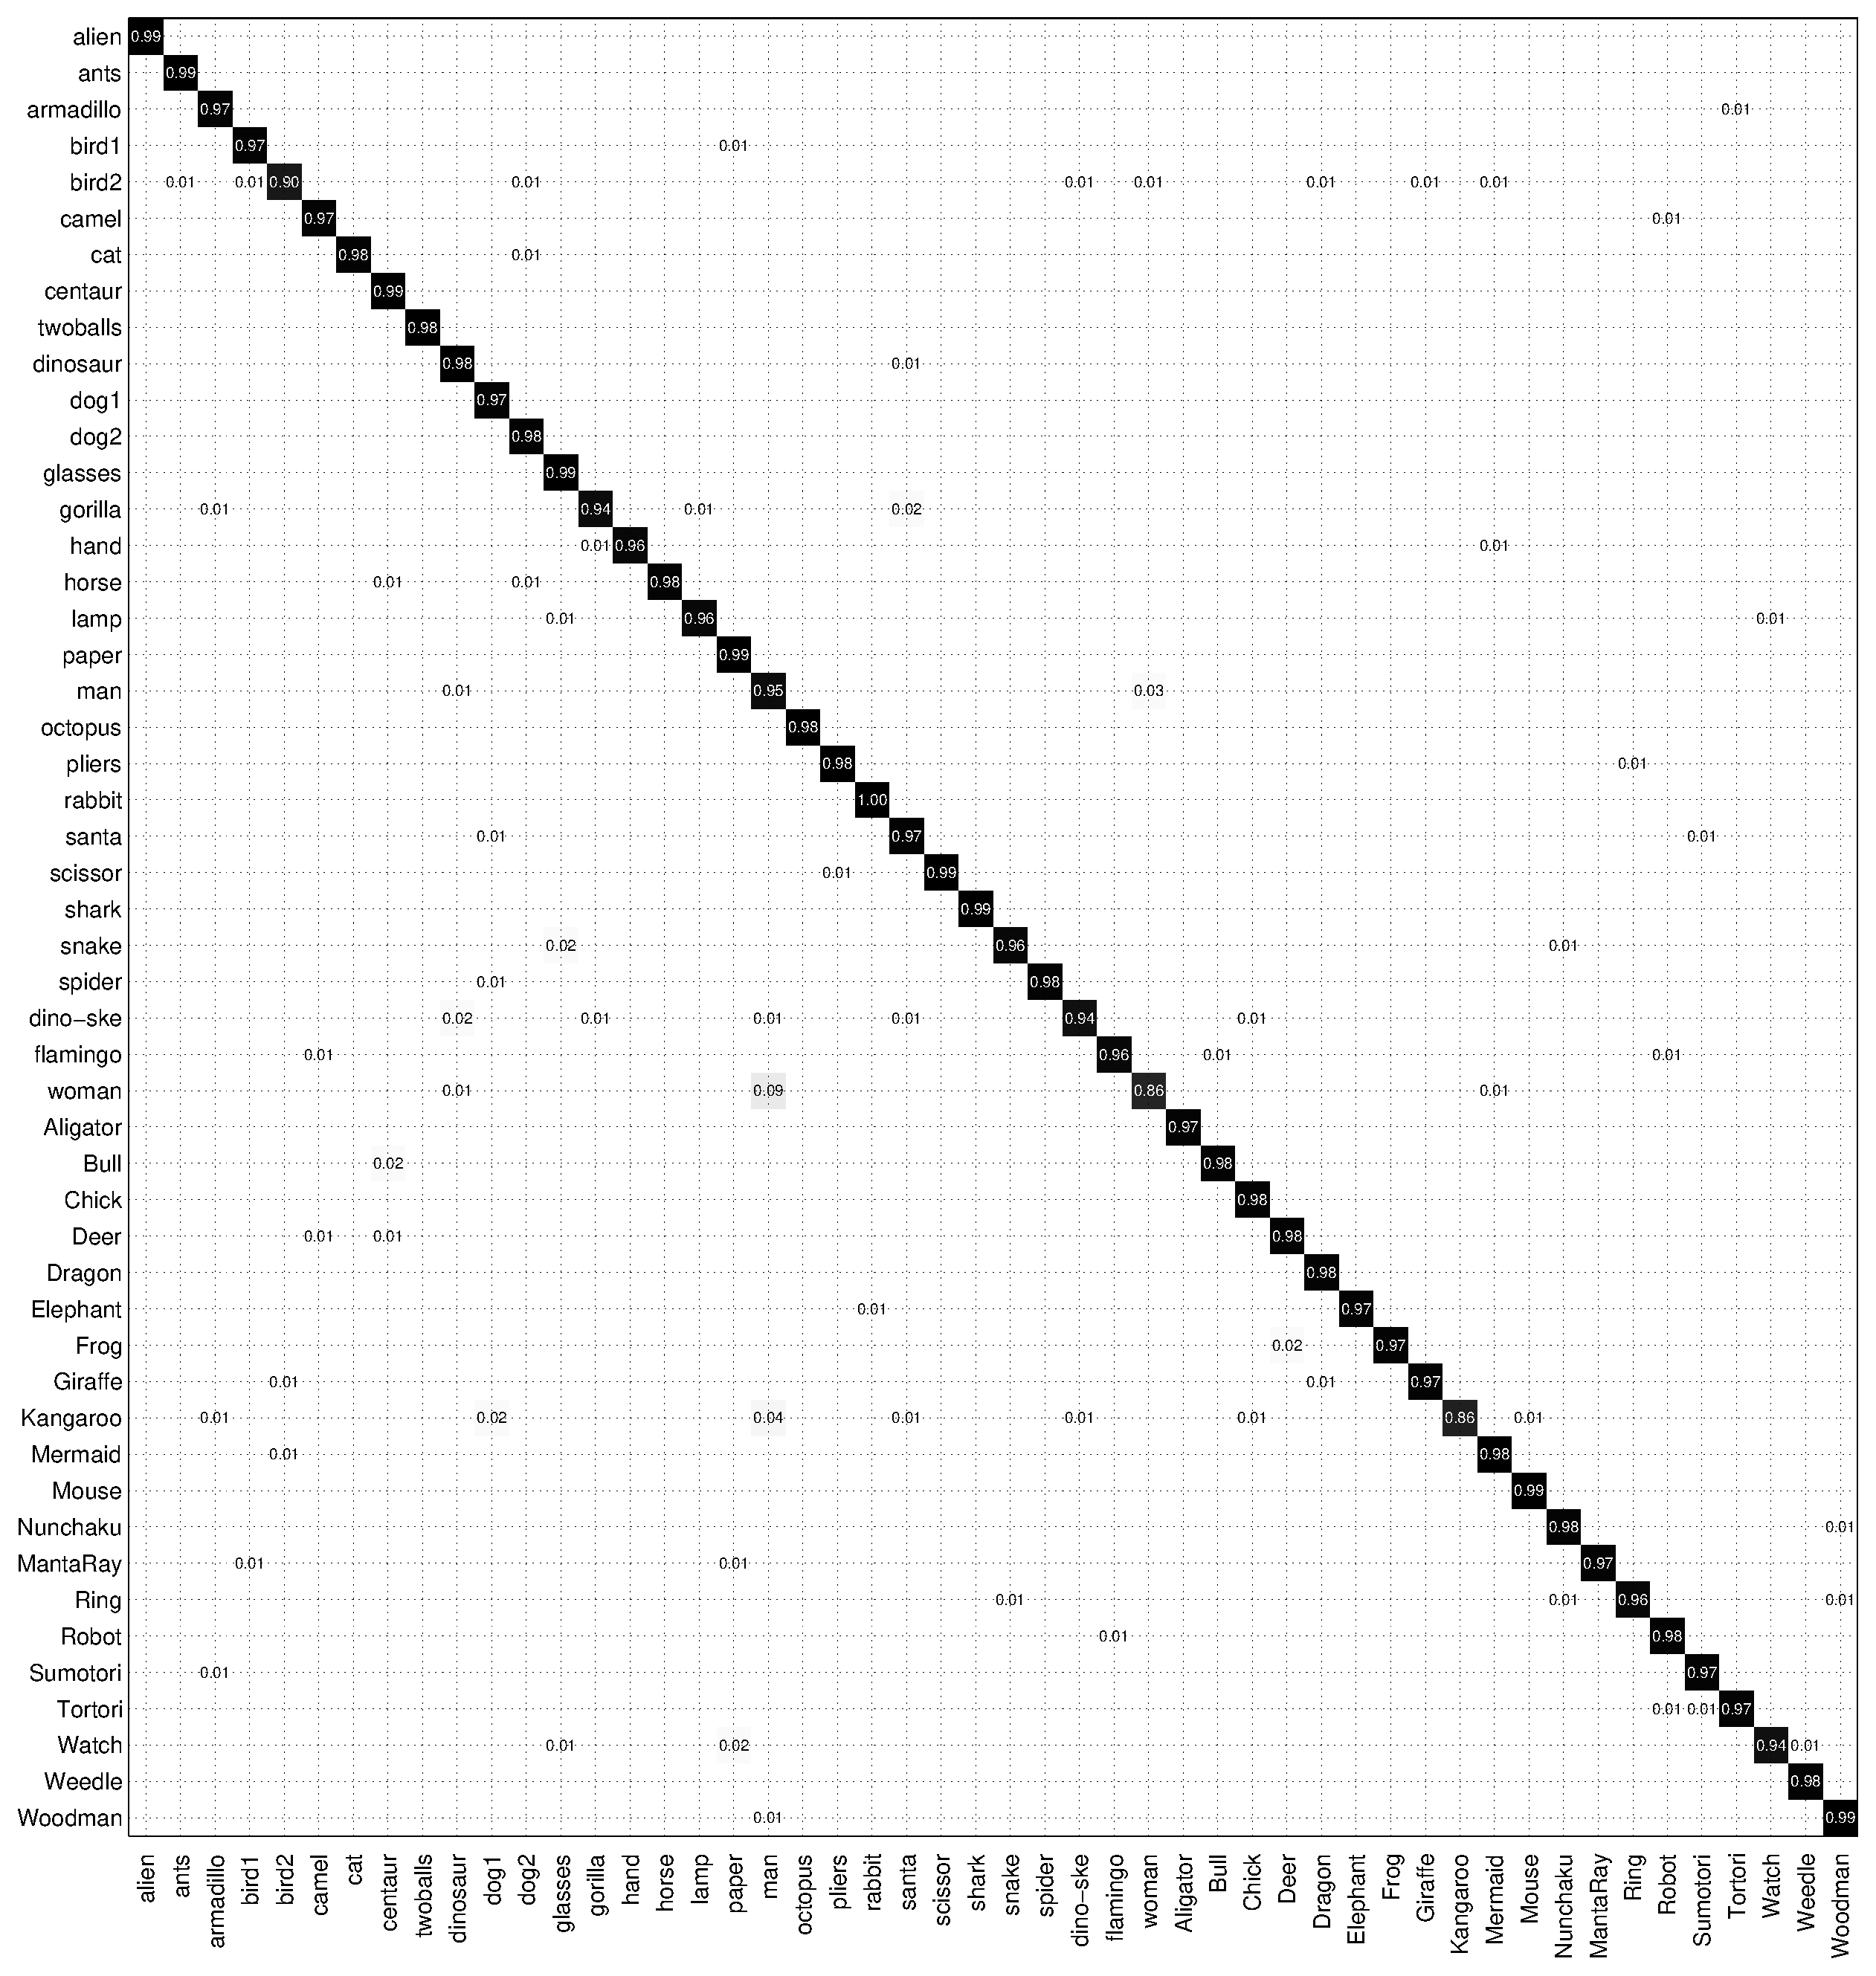
\includegraphics[width=0.45\linewidth]{figures/shrec2015_CM_3view.eps} 
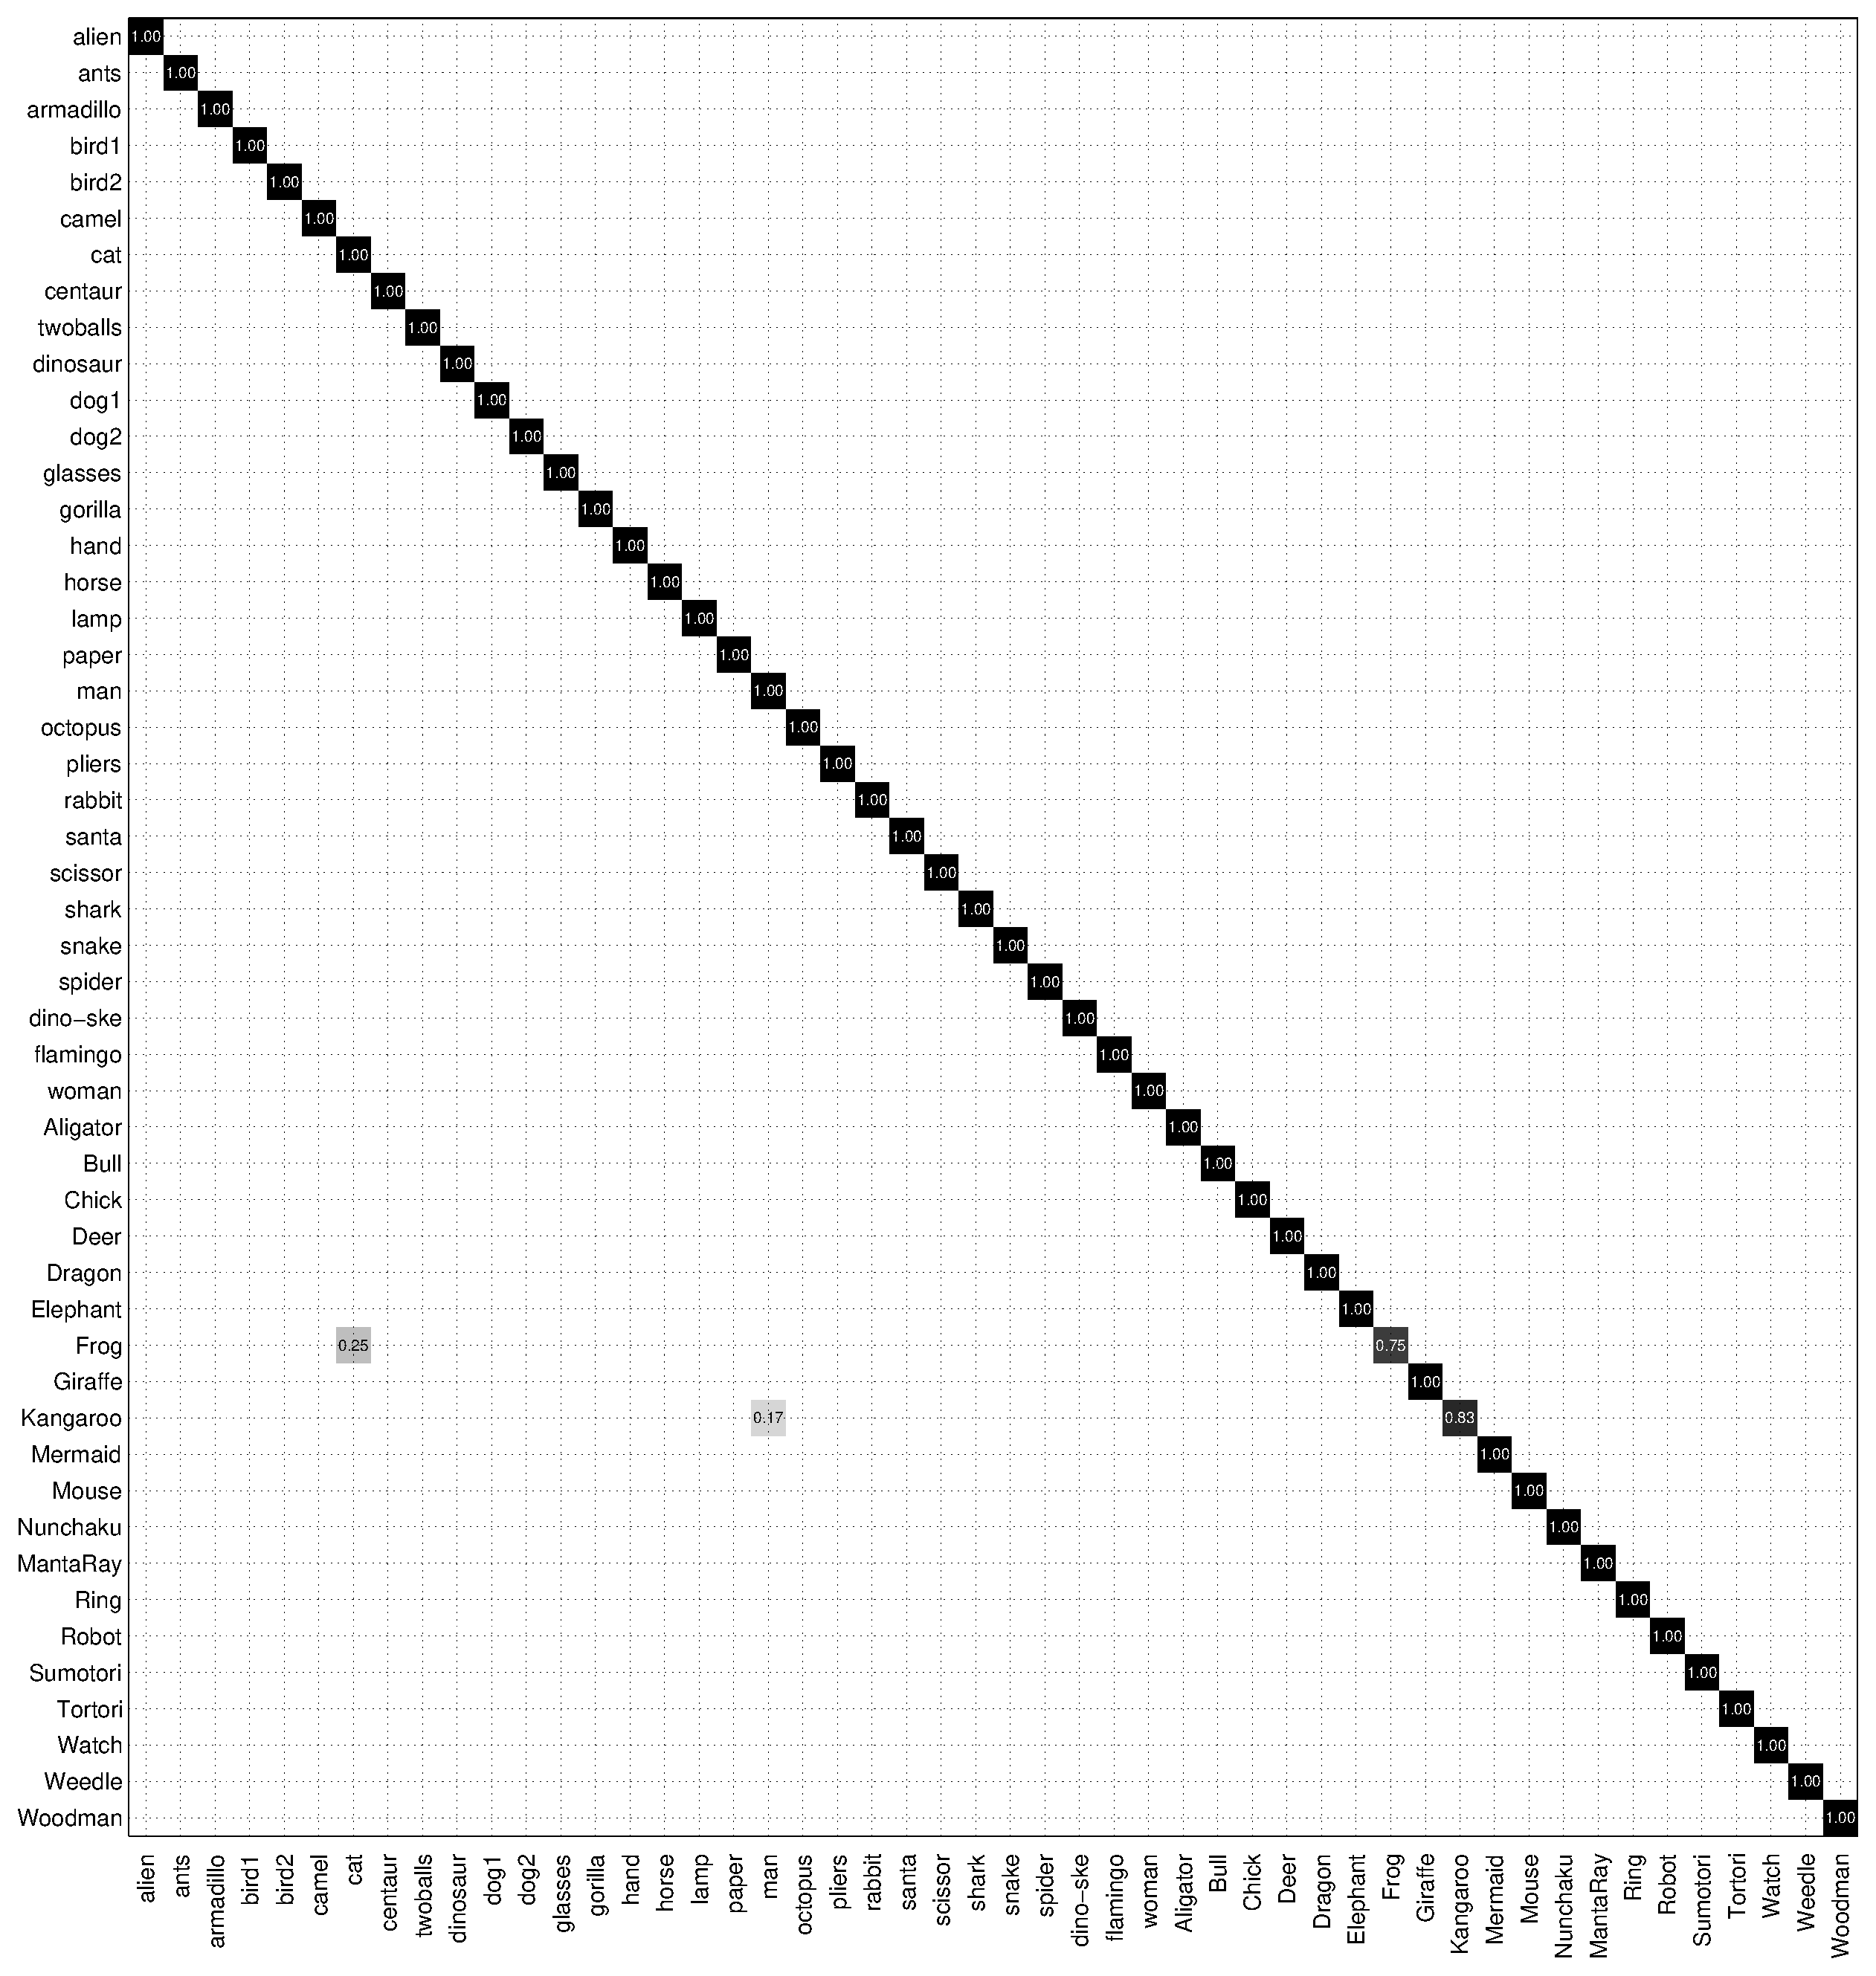
\includegraphics[width=0.45\linewidth]{figures/shrec2015_CM_200view.eps}
\end{center} 
\vspace{-4mm}
\caption{SHREC 2015的3个视图(左)和200个视图(右)的混淆矩阵} \label{fig_cm_shrec2015}
\end{figure*}


在机器学习领域,混淆矩阵是一种特定的表格布局,可以显示算法的性能。混淆矩阵包含有关分类系统完成的实际分类和预测分类的信息。为了进一步详细分析识别结果,使用所提出的方法在四个数据集上进行分类的混淆矩阵中 \ref{fig_cm_shrec2015}。实际上,每一行的总和是一个,因为它们是一个模型,但是,我们只画出了大于0.01的值,这使得一些行的总和不等于$ 1 $。从结果中,我们可以绘制得出的结论是该方法具有广阔的应用前景。横坐标表示实际分类,纵坐标表示预测分类。如图\ref{fig_cm_shrec2015}所示,SHREC 2015数据集混淆矩阵只有3个视图和200个视图。在左图中,虽然错误分类超过了右图,但分类准确性也被接受,因为分类错误的精度非常低。右图中,'猫'的25%被错误分类为'青蛙',同时17% “被误称为”袋鼠“。这种现象可能是由于猫和青蛙产生的一些相似的视图,而“袋鼠”和“人”也是相似的。但平均分类精度接近100%,说明该方法具有广阔的应用前景。
\begin{figure}[tbhp]
\begin{center}
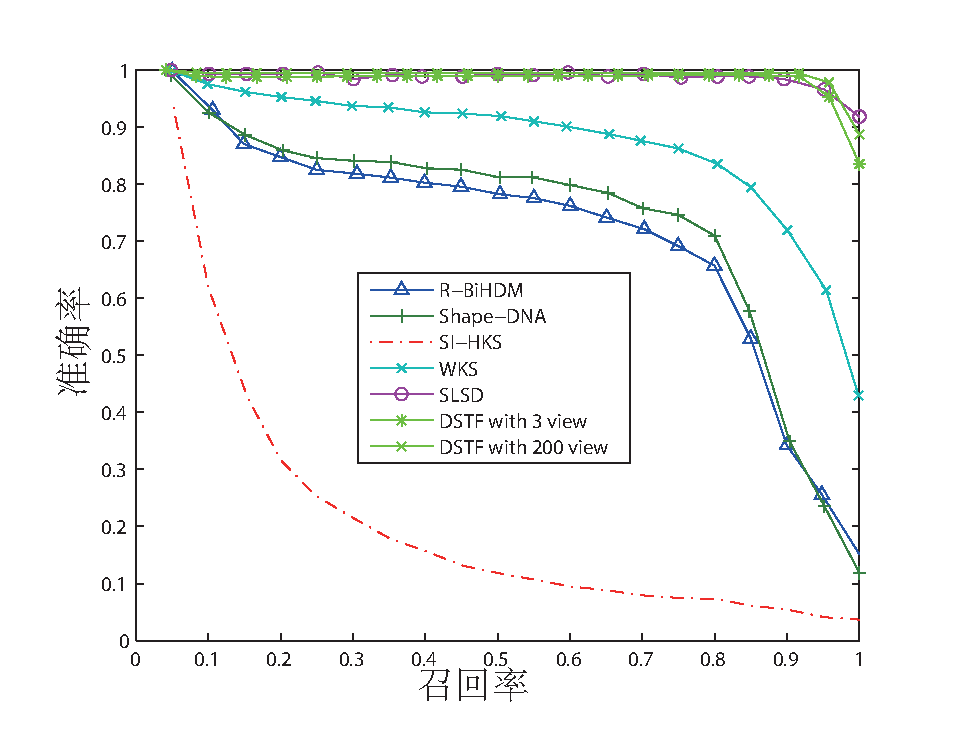
\includegraphics[width=1\linewidth]{figures/all_rp_cl_shrec2015.eps}
\end{center} 
\vspace{-4mm}
\caption{SHREC2015上3视图和200视图的一些最先进的方法和提出的方法的PR曲线。} \label{fig_rp_shrec2015}
\end{figure}




%table
\begin{table}[tbhp]
\caption{采用SHREC2015数据集测量方法对不同方法进行检索性能(\%)} \label{table_retrieval_shrec2015}
\begin{center}
\begin{tabular}{cccccc}  % {lccc} 
\hline  \hline
方法	    						&NN     &FT     &ST     &E      &DCG \\ 
\hline 
HAPT \cite{Giachetti2012Radial} 	&99.8	&96.6	&49.1	&81.5	 &99.2 \\
HKS-TS \cite{Lian2015SHREC}			&6.5	&6.4	&6.2	&7.4	 &39.1 \\
SGWS \cite{Li2013A}					&97.3	&76.0	&40.7   &66.0	 &91.9  \\
EDBCF \cite{Laga2013Geometry}		&97.8	&79.1 	&44.2	&70.8	 &94.3 \\
SLSD	\cite{Hamed2017Nonrigid}	&99.3	&98.0	&49.5	&82.4    &99.4	\\
DSTF 3-views   						&98.6  	&94.2  	&49.1  	&80.6  	 &99.1 \\ 
DSTF 200-views   					&99.5  	&94.9  	&49.4  &81.1  	 &99.6 \\ 
\hline  \hline      
\end{tabular}
\end{center} 
\end{table}

\subsection{检索实验}
对于检索任务,有6个标准评估指标用于评估推荐方法的性能。 它们是 precision-recall curve, nearest neighbor (NN), first tier (FT), second tier (ST), E-measure (E), 和 discounted cumulative gain (DCG),详细的定义可以在\cite{shilane2004princeton}中找到。等式\eqref{cal_cal_distance}被用来描述两个模型之间的相似性。


\textbf {SHREC2015检索实验}。 我们在SHREC2015数据集上进行了检索实验,以评估检索性能。我们的方法和一些现有技术的方法的回想精度曲线绘制在图\ref{fig_rp_shrec2015},其中包括S-HKS\cite {Bronstein2010Scale},WKS\cite{Aubry2011The}和浅层学习形状描述符(SLSD)\cite{Hamed2017Nonrigid}。从图中可以看出,推荐的方法总体上达到了最佳的检索结果。同时,该方法提高了类内相似度,降低了类间相似度。 结果,检索性能得到改善。

表\ref{table_retrieval_shrec2015}列出了我们的方法和一些最先进的方法进行的数值评估结果,包括面积投影变换(HAPT)的直方图\cite {Giachetti2012Radial},HKS-TS \cite {Lian2015SHREC}, SGWS\cite {Li2013A}和EDBCF\cite {Laga2013Geometry}。 从表 \ref {table_retrieval_shrec2015}中,我们可以清楚地看到所提出的方法对于检索是非常好的,这表明STF适合于稀缺的视觉信息获得良好的检索性能。 所提出的方法对于视觉信息稀缺的移动机器人三维识别任务是一种有效的方法。


\begin{figure}[tbhp]
\begin{center}
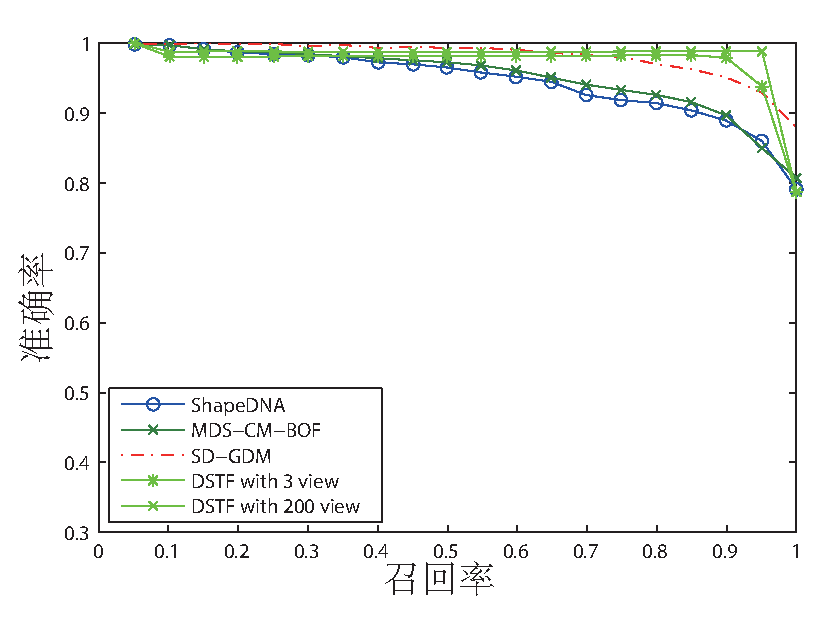
\includegraphics[width=1.0\linewidth]{figures/all_rp_cl_shrec2011.eps}
\end{center} 
\vspace{-4mm}
\caption{SHREC2011上的一些最先进的方法和提出的方法的PR曲线。} \label{fig_rp_shrec2011}
\end{figure}
%table
\begin{table}[tbhp]
\caption{采用SHREC2011数据集测量方法对不同方法进行检索性能(\%)} \label{table_retrieval_results_shrec2011}
\begin{center}
\begin{tabular}{cccccc}  % {lccc} 
\hline  \hline
方法      						&NN &FT &ST &E &DCG\\ 
\hline
Harris3DGeoMap \cite{Lian2011SHREC}	&56.2	&32.5	&23.3	&32.2	&65.4	\\
BOW-LSD \cite{Lavou2011Bag}				&95.5	&67.2 	&40.2	&57.9	&89.7 \\
ShapeDNA \cite{Reuter2006Laplace}		&99.2 	&91.5 	&47.9	&70.5	&97.8	\\
MeshSIFT \cite{Maes2010Feature}		&99.5	&88.4	&48.1	&70.8	&98.0	\\
DSTF	3-views								&97.7	&92.1	&48.7	&71.0	&98.6	\\
DSTF	200-views							&98.7	&93.5	&48.9	&71.4	&99.0	\\
\hline  \hline      % 
\end{tabular}
\end{center} 
\end{table}


\begin{figure}[tbhp]
\begin{center}
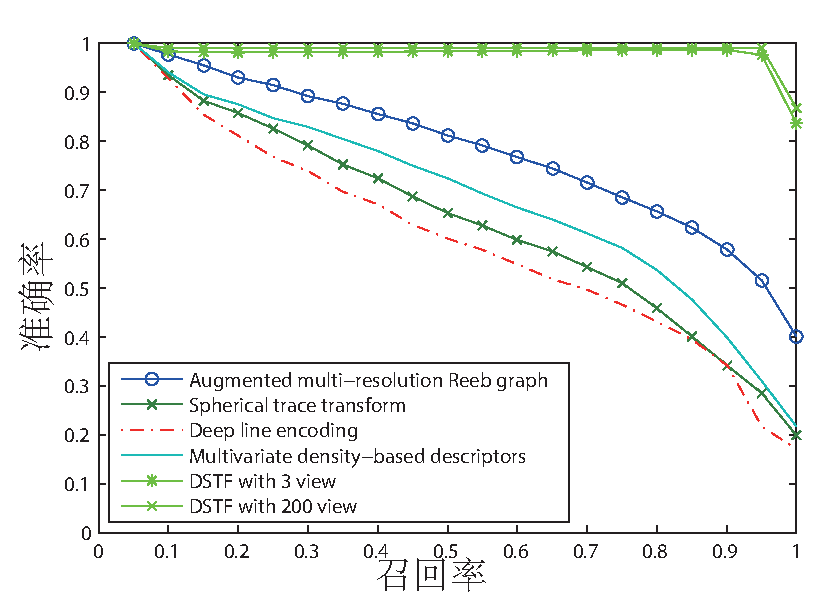
\includegraphics[width=1\linewidth]{figures/all_rp_cl_shrec2007.eps}
\end{center} 
\vspace{-4mm}
\caption{SHREC2007上的一些最先进的方法和提出的方法的PR曲线。} \label{fig_rp_shrec2007}
\end{figure}

%table
\begin{table}[tbhp]

\caption{采用SHREC2007数据集测量方法对不同方法进行检索性能(\%)} \label{table_retrieval_results_shrec2007}
\begin{center}
\begin{tabular}{cccccc}  % {lccc} 
\hline  \hline
方法	    &NN     &FT     &ST     &E      &DCG \\ 
\hline 
DSTF 3-views		&98.3	&92.2	&49.0	&71.4	&98.9	\\
DSTF	200-views	&99.0		&93.8	&49.2	&71.8	&99.3	\\
\hline  \hline      
\end{tabular}
\end{center} 
\end{table}



\begin{figure}[tbhp]
\begin{center}
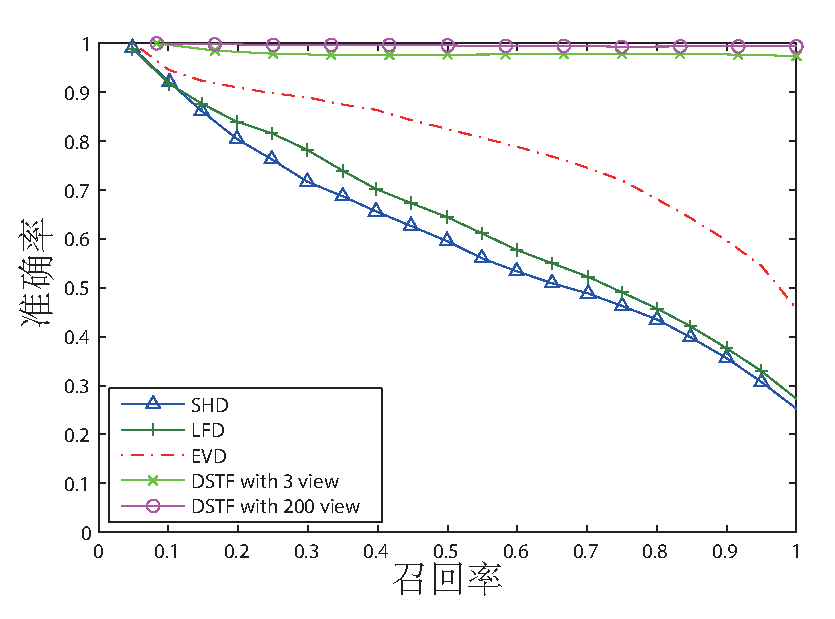
\includegraphics[width=1.0\linewidth]{figures/all_rp_cl_McGill.eps}
\end{center} 
\vspace{-4mm}
\caption{McGill上的一些最先进的方法和提出的方法的PR曲线.} \label{fig_rp_McGill}
\end{figure}

%table
\begin{table}[tbhp]

\caption{采用McGill数据集测量方法对不同方法进行检索性能(\%)}\label{table_retrieval_results_McGill}
\begin{center}
\begin{tabular}{cccccc}  % {lccc} 
\hline  \hline
方法                 &NN &FT &ST &E &DCG\\ 
\hline     
DSTF 3-views					&97.8 &92.9 &48.7 	&81.3		&98.7 \\
DSTF 200-views				&99.8 &	94.9 &49.6	&83.2		&99.7	\\
\hline  \hline      %
\end{tabular}
\end{center} 
\end{table}








\textbf{SHREC 2011, SHREC 2007和McGill检索实验。} 我们还对SHREC 2011,SHREC 2007和McGill数据集进行检索实验,以评估检索性能。我们的方法和一些最先进的方法,包括深度线编码(DLE)\cite {giorgi2007watertight},多元密度描述符(MDD)\cite {giorgi2007watertight},球形轨迹变换(STT )\cite {giorgi2007watertight},增强的多分辨率Reeb图(aMRG)\cite {giorgi2007watertight},ShapeDNA \cite {Reuter2006Laplace},MDS-CM-BOF\cite{lian2010non},SD-GDM \cite{Lian2011SHREC} 球面谐波描述子(SHD)\cite{Kazhdan2003Rotation},光场分布(LFD)\cite{chen2003visual}和EVD \cite {gal2006salient}绘制在图\ref {fig_rp_shrec2011}, \ref {fig_rp_shrec2007}和\ref {fig_rp_McGill}。与这些方法相比,我们的方法要好于其他方法。表\ref {table_retrieval_results_shrec2011},\ref {table_retrieval_results_shrec2007}和\ref {table_retrieval_results_McGill}列出数字评估。结果表明,提出的框架是对于视觉信息稀缺的三维形状进行识别良好效果。


\section{总结}
在本节中,我们提出了一个新的三维形状识别和检索框架,以解决移动机器人面临的信息缺乏的三维形状识别问题。首先,视觉描述符被提取为基于视图的CNNs特征。 然后将不同的视觉描述符作为LSTM的输入,以了解它们之间的顺序关系。 CNN模型就像人类的“视觉系统”一样,从单幅图像中学习视角的特征。 而且,LSTM模型与“记忆系统”类似,挖掘了不同视觉特征的内在时空关系。在分类和检索任务的标准基准上进行的实验已经证明,与最先进的方法相比,推荐的方法实现更好的性能。 实验结果表明,提出的表示方法具有较强的判别能力,能够抑制类内变异,增强类间相似性分离。与传统的计算机视觉形状分析方法不同,我们充分考虑了视觉特性和时空序列特性。 通过使用这种策略,可以对高度非线性的相关性视图模式进行全面建模。

\textbf{局限性。} 我们处理每个视图都是同等重要的,但是有些视图比其他观点重要得多。 最佳视图选择在时空建模中应该被考虑。有限数据集限制了神经网络的规模。 小规模的数据集不能完全训练一个更大的深度学习网络,影响进一步的应用。

\textbf{未来工作。} 首先,目前各视角的权重是相等的,不符合实际。 为了提高所提模型的适应性,应该增加图像权重,从而得到更好的性能。其次,进一步的应用需要更大的神经网络来完成更复杂精细的工作。 因此,有必要建立一个更大的三维形状数据集,以适应更大的深度学习网络。 
